\scanpage{102}
% Archive foliation: 103. Mirror blue show-through belongs to the reverse typescript.
\unsure{(iii)} $\operatorname{gr}u$ est un isom.

\[
\begin{aligned}
u\text{ mono}&\Longrightarrow\operatorname{gr}^0(u)\text{ un mono},&\text{car }\operatorname{gr}^0(u)&\simeq(f^{n-1}A-f^{n-1}B)\\
u\text{ épi}&\Longrightarrow\operatorname{gr}^0(u)\text{ un épi},&\text{car }\operatorname{gr}^0(u)&\simeq(A/fA-B/fB)
\end{aligned}
\]
\[
\operatorname{gr}^0(u)\text{ un mono}\Longleftrightarrow\operatorname{gr}^0(u)\text{ un épi}\Longleftrightarrow\operatorname{gr}^0(u)\text{ un isom}
\]
car $A/fA$ et $B/fB$ de \uline{$=\unsure{\operatorname{rg}}$}.

\[
\operatorname{gr}^0(u)\text{ un isom}\Longrightarrow\operatorname{gr}(u)\text{ un isom}
\]
\margin{car $\operatorname{gr}^i(u)\simeq(\operatorname{gr}^0(u))$ si $0\leq i\leq n-1$}
\[
\operatorname{gr}(u)\text{ un isom}\Longrightarrow u\text{ un isom}.
\]
\margin{bien connu.}

\uline{Cor.} \deleted{\unsure{Soit}} Pour \unsure{$\forall$} entier $0\leq i\leq n$, $f^iA$ est le seul sous-objet de \unsure{T.A} \inserted{$B$} de $A$, de hauteur $n-i$ et de rang $\rho$ : en effet, un tel $B$ est contenu dans $f^iA=\operatorname{Ker}f^{n-i}$, et d'après ce qui précède, lui est égal.

\uuline{Cor.} dual : $A/f^{n-i}A$ est le seul objet quotient de $A$ qui soit de Tate, de hauteur $n-i$, de rang $\rho$.

\figure{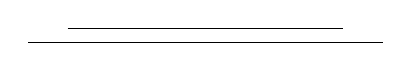
\begin{tikzpicture}\draw (0,0)--(3.5,0);\draw (-.5,-.18)--(4,-.18);\end{tikzpicture}}

$G$ schéma en groupes commutatifs, plat \deleted{\unsure{loc}} de présentation finie sur $S$. Un endom $f$, et entier $n$ tel que $f^n=0$. Soit $1\leq j\leq n-1$ fixé.

Conditions équivalentes

(i) [$\operatorname{Ker}f^j$ est plat, et] \deleted{\unsure{morphisme}} $f^{n-j}:G-\operatorname{Ker}f^j$ est fid \deleted{plat}.

(ii) $\forall s\in S$, $(G_s,f)$ est un objet de \unsure{T.A} de \deleted{\unsure{long}} hauteur $n$ (dans la catégorie des groupes algébriques commut sur $k$).
